\chapter{Heavy Ion Detection}
\section{Kinematics}
In HELIOS, light ions are detected at essentially a fixed radius---$\rho_0$ the radius of the detector array---over a range of $z$.  However, this detection scheme is not typically suitable for the heavy ion reaction products which are emitted over a narrow range of angles and due to their rigidity, only go through a fraction of the helical orbit.  Instead, a detector is placed at a fixed $z$, measuring heavy ion reaction products over a range of $\rho$.  The kinematics of the light ion reaction product as they relate to the silicon detector array have been discussed in Chapt.~\ref{HELIOS_Concept}.  This chapter discusses the relevant kinematics of the heavy ion reaction product and a number of heavy ion detector approaches.  The acceptance of a given detector system is related to the radial excursion and angle of rotation of the heavy ion products, discussed below.
\subsection{Excursion}

\begin{figure}%
\centering
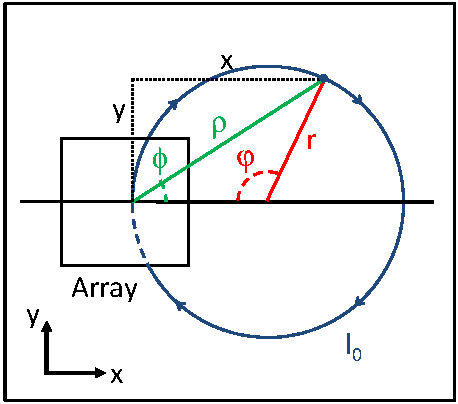
\includegraphics[width=\columnwidth,height=0.33\textheight,keepaspectratio]{orbit_coord}%
\caption[Illustration of the relationship between orbit-centric and array-centric coordinates]{Illustration of the relationship between the orbit-centric coordinates ($r$,$\varphi$) and the array-centric coordinates ($\rho$,$\phi$) or ($x$,$y$), as viewed in the transverse plane of the solenoid.}%
\label{orbit_coord}%
\end{figure}

The radial excursion $\rho$ of a particle orbit is expressed in term of the angle of rotation through the orbit of the particle.  Here let us define two angles of rotation, as illustrated in Fig.~\ref{orbit_coord}.  The position of the particle % orbit
in the transverse plane of the solenoid, relative to the fixed solenoid axis, can be written as ($x$,$y$) or ($\rho$,$\phi$), where $\phi$ is the angle of rotation.  These are the same coordinates defined in \S\,\ref{coord}.  For a given particle orbit, the angle of rotation about the orbit's center is written as $\varphi$.  In this notation, the path length of an orbit is written as $l_0=\varphi r$ and the radial excursion is given as a function of orbit-centric rotation angle.

\begin{equation}
\begin{split}
\rho&=\sqrt{y^2+x^2}\\
&=\sqrt{r^2\sin^2(\varphi)+(r-r\cos(\varphi))^2}\\
&=\sqrt{r^2\sin^2(\varphi)+r^2+r^2\cos^2(\varphi)-2r^2\cos(\varphi)}\\
&=\sqrt{2r^2-2r^2\cos(\varphi)}\\
&=r\sqrt{2-2\cos(\varphi)}
\end{split}
\label{eq:radius}
\end{equation}
With the definition given in Eq.~\ref{eq:radius}, $\rho(0)=0$ corresponds to the beginning of the orbit and the maximum excursion is given by $\rho(\pi)=2r$.  This equation in plotted as a function of $z$ in Figs.~\ref{luminos} and \ref{sim_traj}.

\subsection{Rotation}
The angle $\varphi$ can be written as a function of the axial position $z$

\begin{equation}
\begin{split}
\varphi&=\frac{t}{T_\mathrm{cyc}}2\pi\\
&=t\omega_c\\
&=\frac{z}{v_\parallel}\omega_c
\end{split}
\label{eq:rot}
\end{equation}
where $\omega_c$ is the cyclotron frequency of the ion.  This expression can be %further 
rewritten as a function of the emission angle by using Eq.~\ref{eq:vpara}.

With reference to Fig.~\ref{orbit_coord}, the angle of rotation relative to the solenoid axis $\phi$ can be written in terms of the orbit-centric rotation angle $\varphi$ and orbit radius $r$.  In formulating this relationship, one encounters a half-angle identity which simplifies the relationship as follows:
\begin{equation}
\begin{split}
\phi&=\arctan \left(\frac{y}{x}\right)\\
\tan(\phi)&=\frac{r\sin(\varphi)}{r-r\cos(\varphi)} \qquad \textrm{half-angle identity}\\
\phi&=2\varphi. 
\end{split}
\label{eq:angles}
\end{equation}
Substituting Eq.~\ref{eq:rot} into Eqs.~\ref{eq:radius} and \ref{eq:angles} allows the calculation of the radial excursion $\rho$ and rotation angle $\phi$ as a function of the axial position. 

\section{Silicon Array}
The heavy ion detector array used in Refs.~\cite{Schiffer_2010,Wuosmaa_2010} is shown in Fig.~\ref{recoil}. This is also the same heavy recoil array used in non-solenoidal (traditional) detector schemes as in Ref.~\cite{Lee_2010}.  The array consists of four sets of two quadrant detectors arrayed in a $\Delta E$-$E$ configuration, discussed below.  The silicon detectors are Design QQQ1 single area pad detectors manufactured by Micron Semiconductor.  The typical thickness of the $\Delta E$ detector is in the range of 75--500\,$\mu$m, depending on the reaction being studied, and the thickness of the $E$ detector is typically in the range of 500--1500\,$\mu$m.  The PC board on which the detectors are mounted covers 90$^\circ$, while the silicon detectors themselves cover $82^\circ$.  The active area of the silicon detectors has an inner radius of 9.0\,mm and an outer radius of 50.0\,mm, for a total active area of 1731.0\,mm$^2$ per detector.  For the measurements reported in Refs~\cite{Schiffer_2010,Wuosmaa_2010}, the heavy recoil array was mounted to the center of the downstream alignment ring, %active area of the $\Delta E$ detector was 
at a fixed position of $z=+1,032$\,mm.

\begin{figure}[ht]
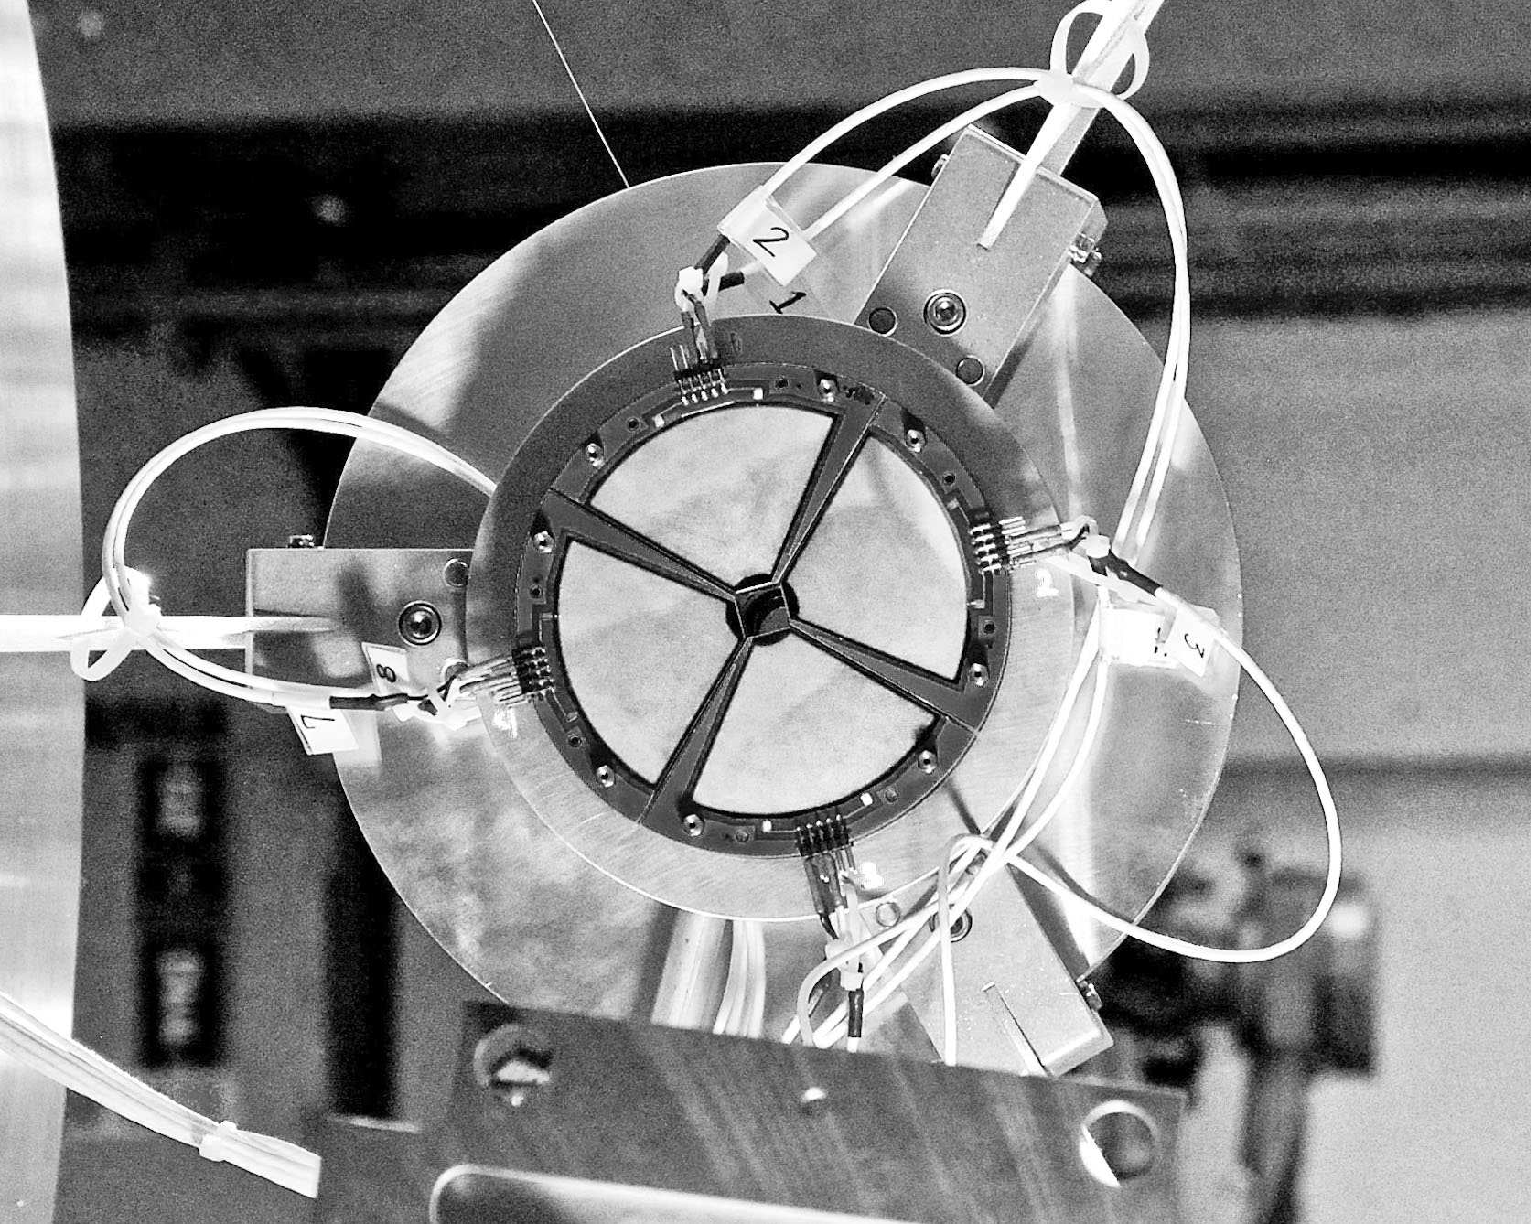
\includegraphics[width=\columnwidth,height=0.5\textheight,keepaspectratio]{DSC_0610}%
\caption[The heavy recoil detector array telescope installed on the downstream alignment ring]{The heavy recoil detector array telescope installed on the downstream alignment ring.  The array has been rotated in the plane of the photograph (azimuthally) to optimize the phase-alignment (discussed in the text) of the heavy recoil orbits to that of the ejectiles.  Photo by A.~H.\ Wuosmaa, \photodate\formatdate{24}{2}{2009}}
\label{recoil}%
\end{figure}

\begin{figure}
\centering
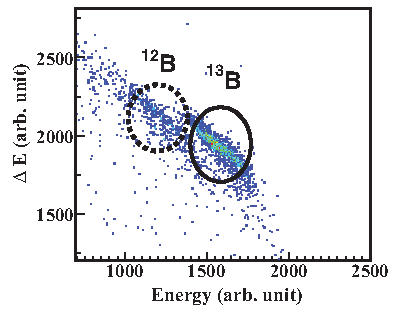
\includegraphics[height=0.33\textheight,width=\columnwidth,keepaspectratio]{Lee_2010_fig1c}%
\caption[Heavy ion $\Delta E$-$E$ particle identification spectrum from the $^{12}$B($d$,$p$)$^{13}$B reaction]{Heavy ion $\Delta E$-$E$ particle identification spectrum from the $^{12}$B($d$,$p$)$^{13}$B reaction.  Figure from Ref.~\cite[Fig.~1(c)]{Lee_2010}.}%
\label{B12_PID}%
\end{figure}

\subsection{Principle}
The heavy ion is identified by an energy loss measurement.  The front detectors (visible in the figure) are selected to be thin compared to the stopping range of the incident particles.  With this configuration, the incident particles do not deposit their total energy in the $\Delta E$ detector.  Instead, in incident particles are transmitted through the $\Delta E$ detector, losing a fraction of their total energy.  The residual energy of the incident particle is then deposited in the $E$ detector which is selected to be thick enough to stop the incident particles.  The expression that describes the energy loss is known as the \textit{Bethe formula}; at low energy (non-\-relativistic velocities), the equation takes the form
\begin{equation}
-\frac{dE}{dz}=4\pi e^4 n\frac{ Z^2}{m v^2} \left(\ln \frac{2mv^2}{I}\right)\qquad \textrm{Bethe formula}
\label{bethe}
\end{equation}
where $n$ is the electron density of the absorber; $m$, $v$, and $Z$  are the mass, velocity, and atomic number of the incident particle, respectively; and $I$ is the average ionization potential of the absorber---in this case, the silicon detector.  When $I$ is given as a function of $Z$, the atomic number of the absorber material, Eq.~\ref{bethe} is referred to as the \textit{Bethe-Bloch formula}.  The parameter $I$ is typically determined experimentally for each element or detector type.  The Bethe formula may be rewritten without a loss of generality as

\begin{equation}
\frac{dE}{dz}=C_1 \frac{mZ^2}{E} \ln C_2 \frac{E}{m}
\label{bethe_simp}
\end{equation}
where the parameters relating to the detector material have been replace by the constants $C_1$ and $C_2$~\cite{Knoll_1979}.  

Due to the quasi-elastic nature of direction reactions, the heavy ion reaction products corresponding to different transitions have nearly the same energy.  However, for a narrow range of incident particle energy, Eq.~\ref{bethe_simp} shows that the energy loss in fixed thickness of the transmission detector ($\Delta E$)  scales roughly with $mq^2$, which allows for the separation of reaction products.  Fig.~\ref{B12_PID} the characteristic heavy ion particle identification spectrum from Ref.~\cite{Lee_2010} which plots the energy loss in the $\Delta E$ detector versus the residual energy in the $E$ detector.  The figure shows that the reaction products from $d$($^{12}$B,$p$)$^{13}$B have been separated, with the dashed ellipse indicating the loci corresponding to $^{12}$B and the solid ellipse indicating $^{13}$B.  The presence of $^{12}$B in the spectrum is due to the in-flight $n$-decay of the recoiling $^{13}$B nucleus.  Although this spectrum was obtained in a ``traditional'' detector setup, the detection principle is the same and the resulting spectrum is the same as those obtained with HELIOS~\cite{Schiffer_2010}.

\subsection{Alignment}
Each of the recoil detectors covers an azimuthal range of $\Delta \phi = 0.46\pi$, while the range covered by each detector in the silicon detector array is  $\Delta \phi = 0.24\pi$.  A corollary of this configuration is that each detector array has rotationally symmetric dead areas separated by 90$^\circ$; this dead area is 0.26$\pi$ wide for the silicon detector array and 0.14$\pi$ wide for the heavy recoil detector array.  This relationship is displayed in Fig~\ref{fig_phase} which shows the simulated detector yields for both arrays.  In this figure, the arrays have been aligned such that active area of each array is centered relative to one another.  However, in this configuration it is not guaranteed that a particle detected in the active area of one array will have its corresponding reaction product intercept an active area of the other array.  Therefore, the detector arrays must be aligned azimuthally so that coincident events may be detected.

The description of particle orbits discussed in this chapter applies to both the light ion ejectile and the heavy ion recoil.  In an experimental setup, the heavy recoil array would be rotated azimuthally (see Fig.~\ref{recoil}) to maximize its measured yield and thus maximize the measured coincidences between the arrays.  This procedure of determining the optimal phase-alignment of the detector arrays can be accomplished with simulations or analytic calculation.  Take as an example the $^{12}$B($d$,$p$) reaction at a bombarding energy of 6.24\,\AMeV, a central field of 1.04\,T in HELIOS, and a target-to-detector separation of $\Delta z=369$.  The light ion ejectiles---protons, in this case---corresponding to transitions to the 3.48\,MeV state in $^{13}$B rotate through an average angle of $\Delta \varphi=348^\circ$ ($\Delta \phi=186^\circ$) before being detected by the silicon detector array.  For the purposes of alignment, this angle of rotation can be taken as intercepting the center of a given detector on the silicon detector array.  Therefore, the corresponding heavy ion recoil should intercept the center of a detector element (41$^\circ$ from the active edge) on the heavy recoil array for optimal alignment.

If the light ion ejection is taken as being emitted at an angle of $\phi_0$, the heavy recoil is ejected at an angle of $\phi_0+180^\circ$ and is detected at an angle of $\phi_0+180^\circ-\varphi/2$.  In this example, the recoiling $^{13}$B ions rotate through an angle of $\Delta \varphi=77.1^\circ$ before hitting the heavy 
recoil detector located at $z=+1032$\,mm.  This angle of rotation is equivalent to a difference in axial rotation (phase difference) of $41.8^\circ$.  Therefore, the heavy
 recoil should be rotated $-0.8^\circ\pm 21^\circ$.  For the actual experiment, the array was
  rotated 15$^\circ$, which is within this range.  The optimal position has such a large range because of the heavy recoil array has about twice the azimuthal coverage of the silicon detector array.

\begin{figure}%
\centering
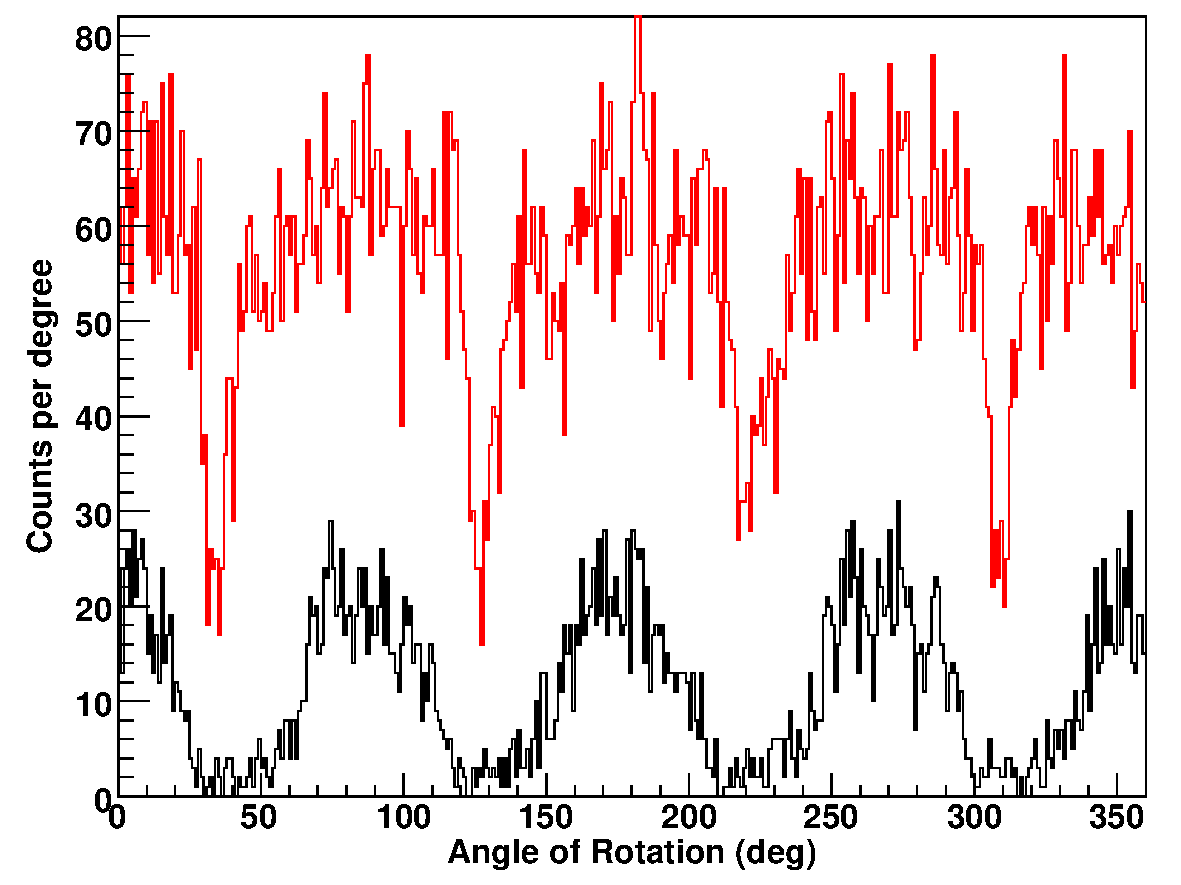
\includegraphics[width=\columnwidth,height=0.33\textheight,keepaspectratio]{cPhiCov}%
\caption[Simulated detector array yields illustrating the azimuthal coverage of each array]{(color online) Simulated detector array yields illustrating the azimuthal coverage of each array.  The silicon detector array (black) is in its normal orientation with the top of the detector array centered at 90$^\circ$ (vertical).  The heavy recoil detector (gray/red) has been rotated so that the center of each detector is aligned with the corresponding detector element on the silicon detector array to illustrate the azimuthal coverage of each array.  }%
\label{fig_phase}%
\end{figure}

\section{Ionization Chambers}
As the mass of the incident heavy recoil increases, an increasingly thin $\Delta E$ detector is needed in order to allow the transmission for the incident particle.  Also, as the thickness of the $\Delta E$ detector decreases, the uniformity of the detector thickness becomes increasingly important.  Furthermore, the radiation damage in a silicon detector increases dramatically for heavy ions in the mass range of typical fission fragments~\cite{Knoll_1979}.  An alternate approach to using semiconductor detectors which is suitable for heavy ion measurements is the use of gas-filled ionization chambers.  As of this writing, a new heavy recoil detector array is being characterized for use in HELIOS.

The new heavy recoil detector array consisting of two gas-filled ionization detector components.  The arrangement of the new detectors is shown in Fig.~\ref{bragg}.  The first component of the array is a large area parallel-plate avalanche counter (PPAC).  This type of detector is based on two closely-spaced parallel electrode plates which are held at high voltage.  The gap between the plates is filled with an ionizing gas and the voltage between the plates is selected so that the gas is near breakdown, \textit{i.e.} the avalanche regime.  This detector is ideal for providing timing information and a grid of anode wires provides position information.  Since the incident heavy ions fully pass through the PPAC detector, this is the gas-filled analogue of the $\Delta E$ detector.  However, in avalanche mode, the energy resolution is only about $\delta E/E = 20$\%.
%\subsection{Bragg Curve Detector}

The second component of the heavy ion detector is a Bragg curve detector which was used in a previous application \cite{Pearson_1995}.  Fig.~\ref{bragg} shows a photograph of this detector being characterized next to the HELIOS spectrometer.  The Bragg curve detector is a ionization chamber which is filled with gas at a sufficient pressure ($\approx 50$\,mbar) to stop the incoming heavy ions.  The detector has an active area of 24\,cm long and 14.4\,cm in diameter.  The residual energy $E$ of the incident ions is measured as well as the position profile of the energy loss.  The energy loss profile is known as the Bragg curve (hence the name of the detector) and position of the peak of the cure allows for $q$-identification of the incident particles.
\begin{figure}[hb]
\centering
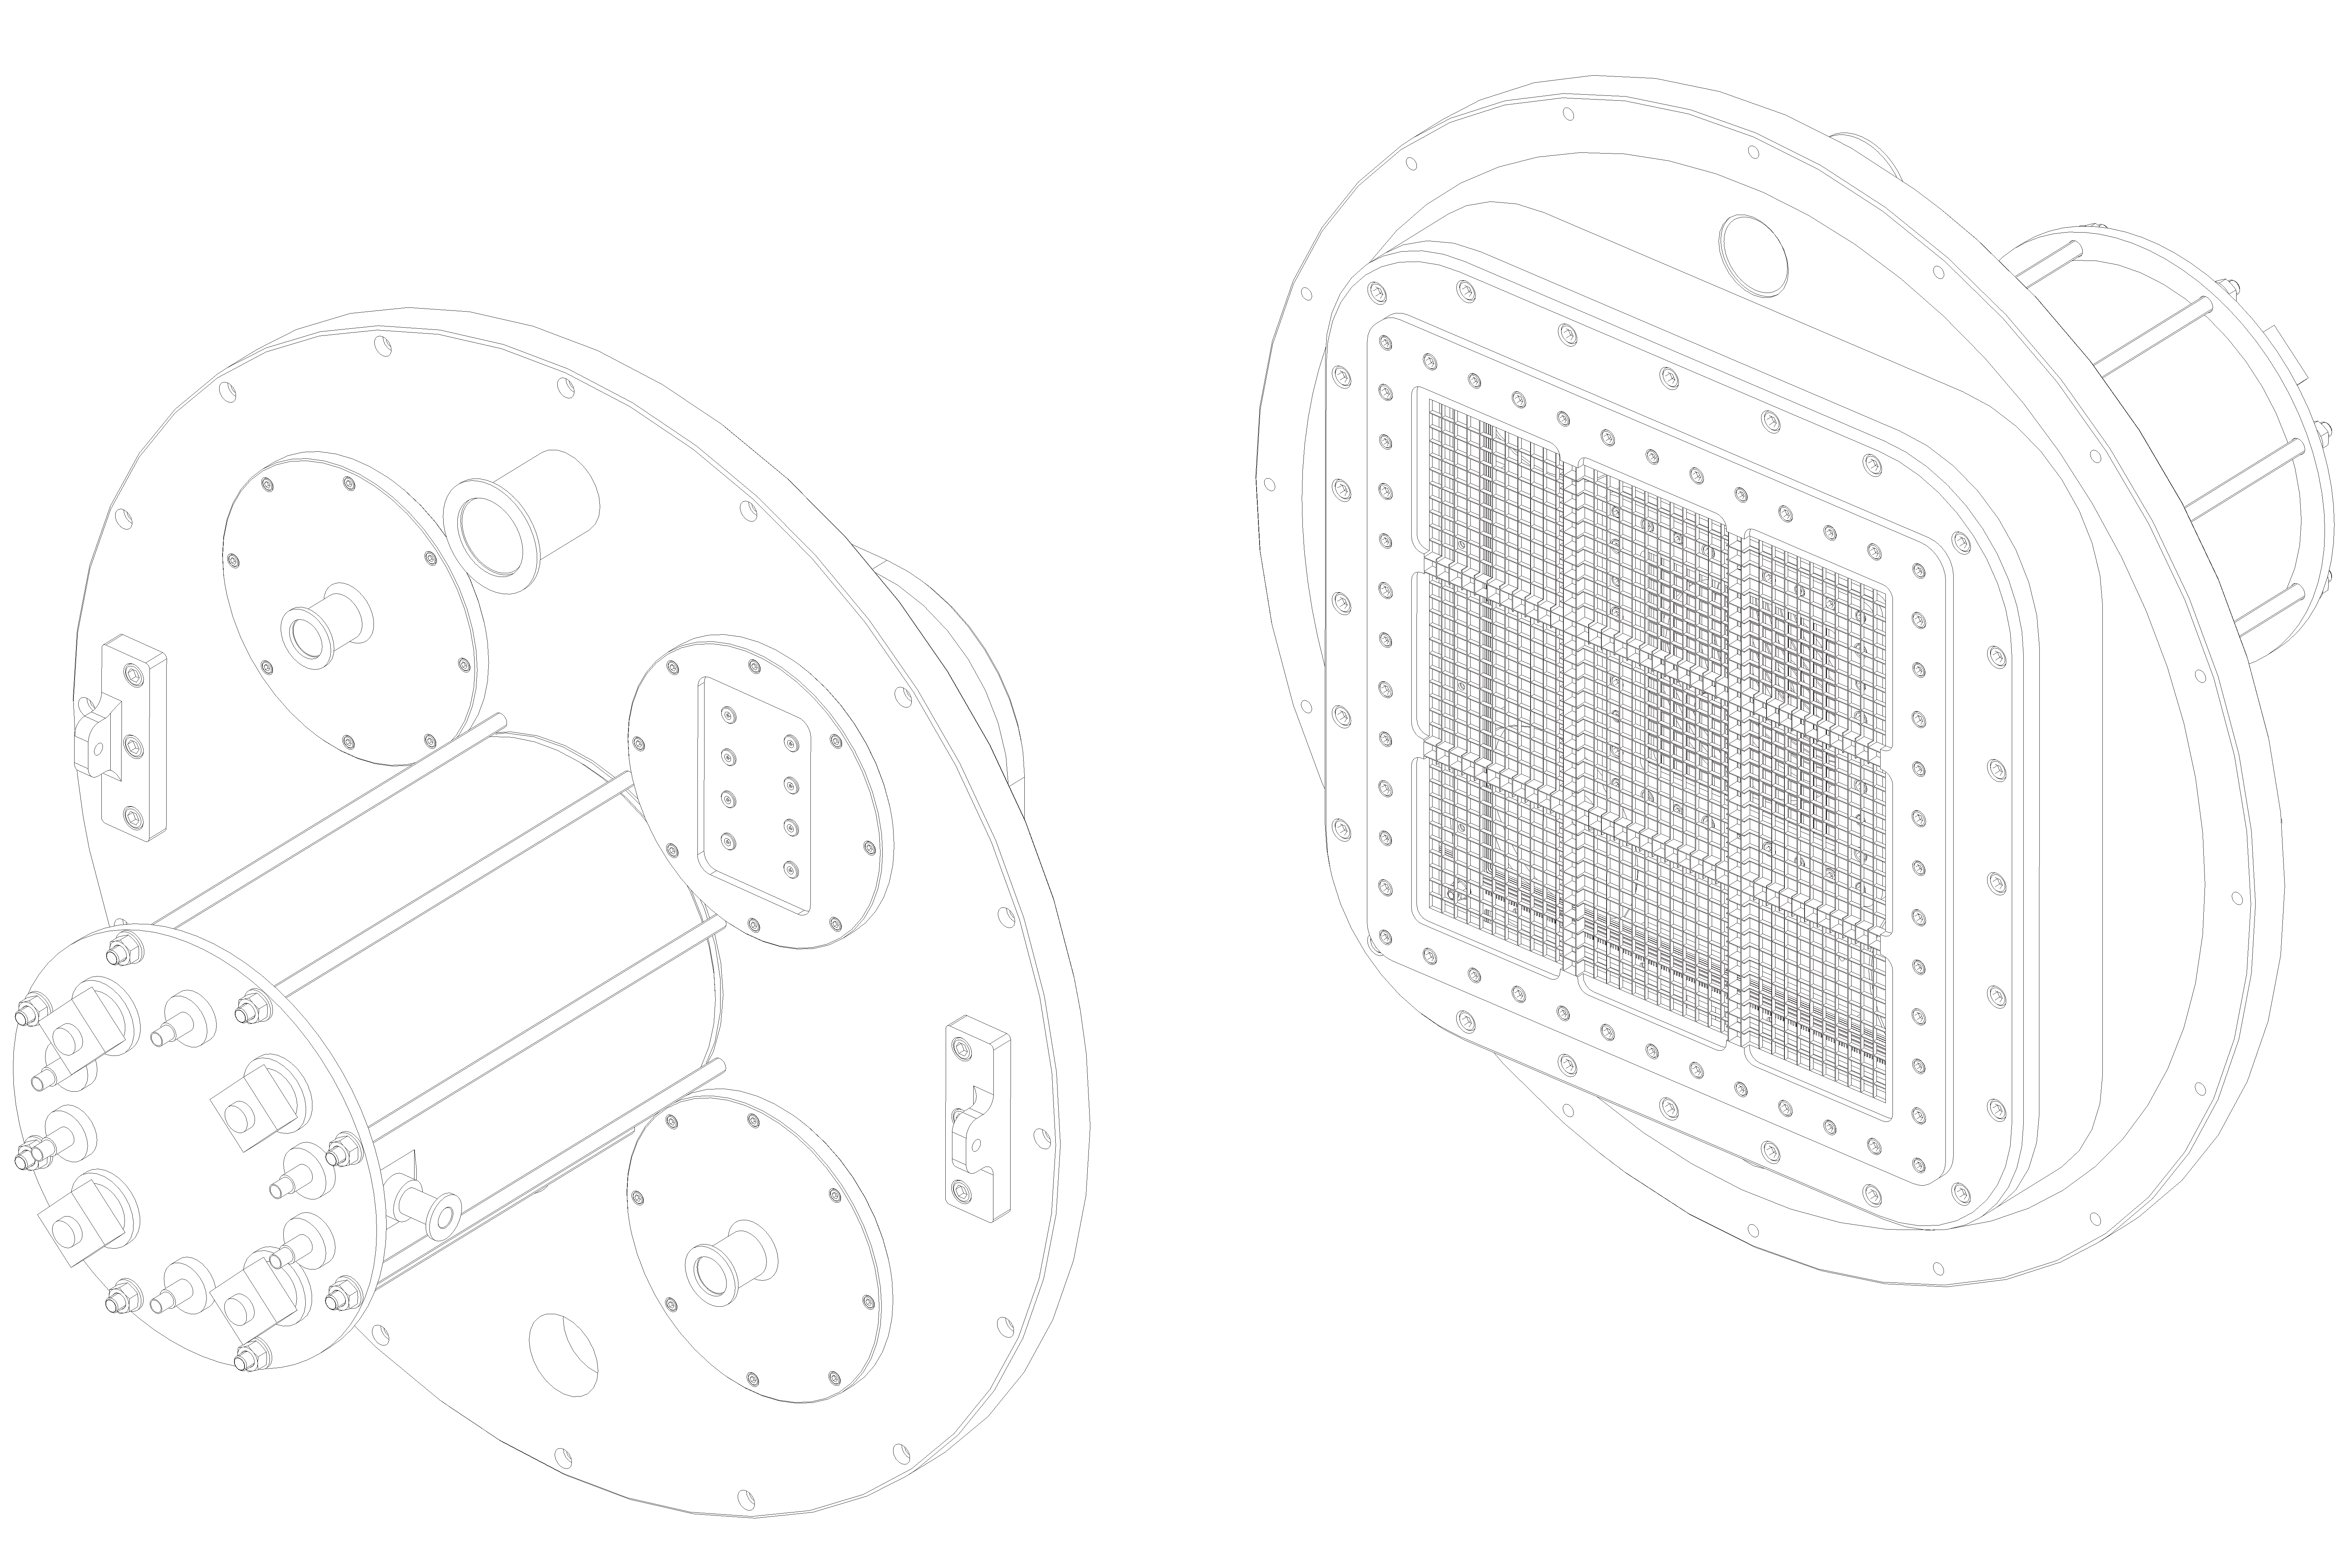
\includegraphics[width=0.45\textwidth,height=0.3\textheight,keepaspectratio]{door}\hspace*{\stretch{1}}
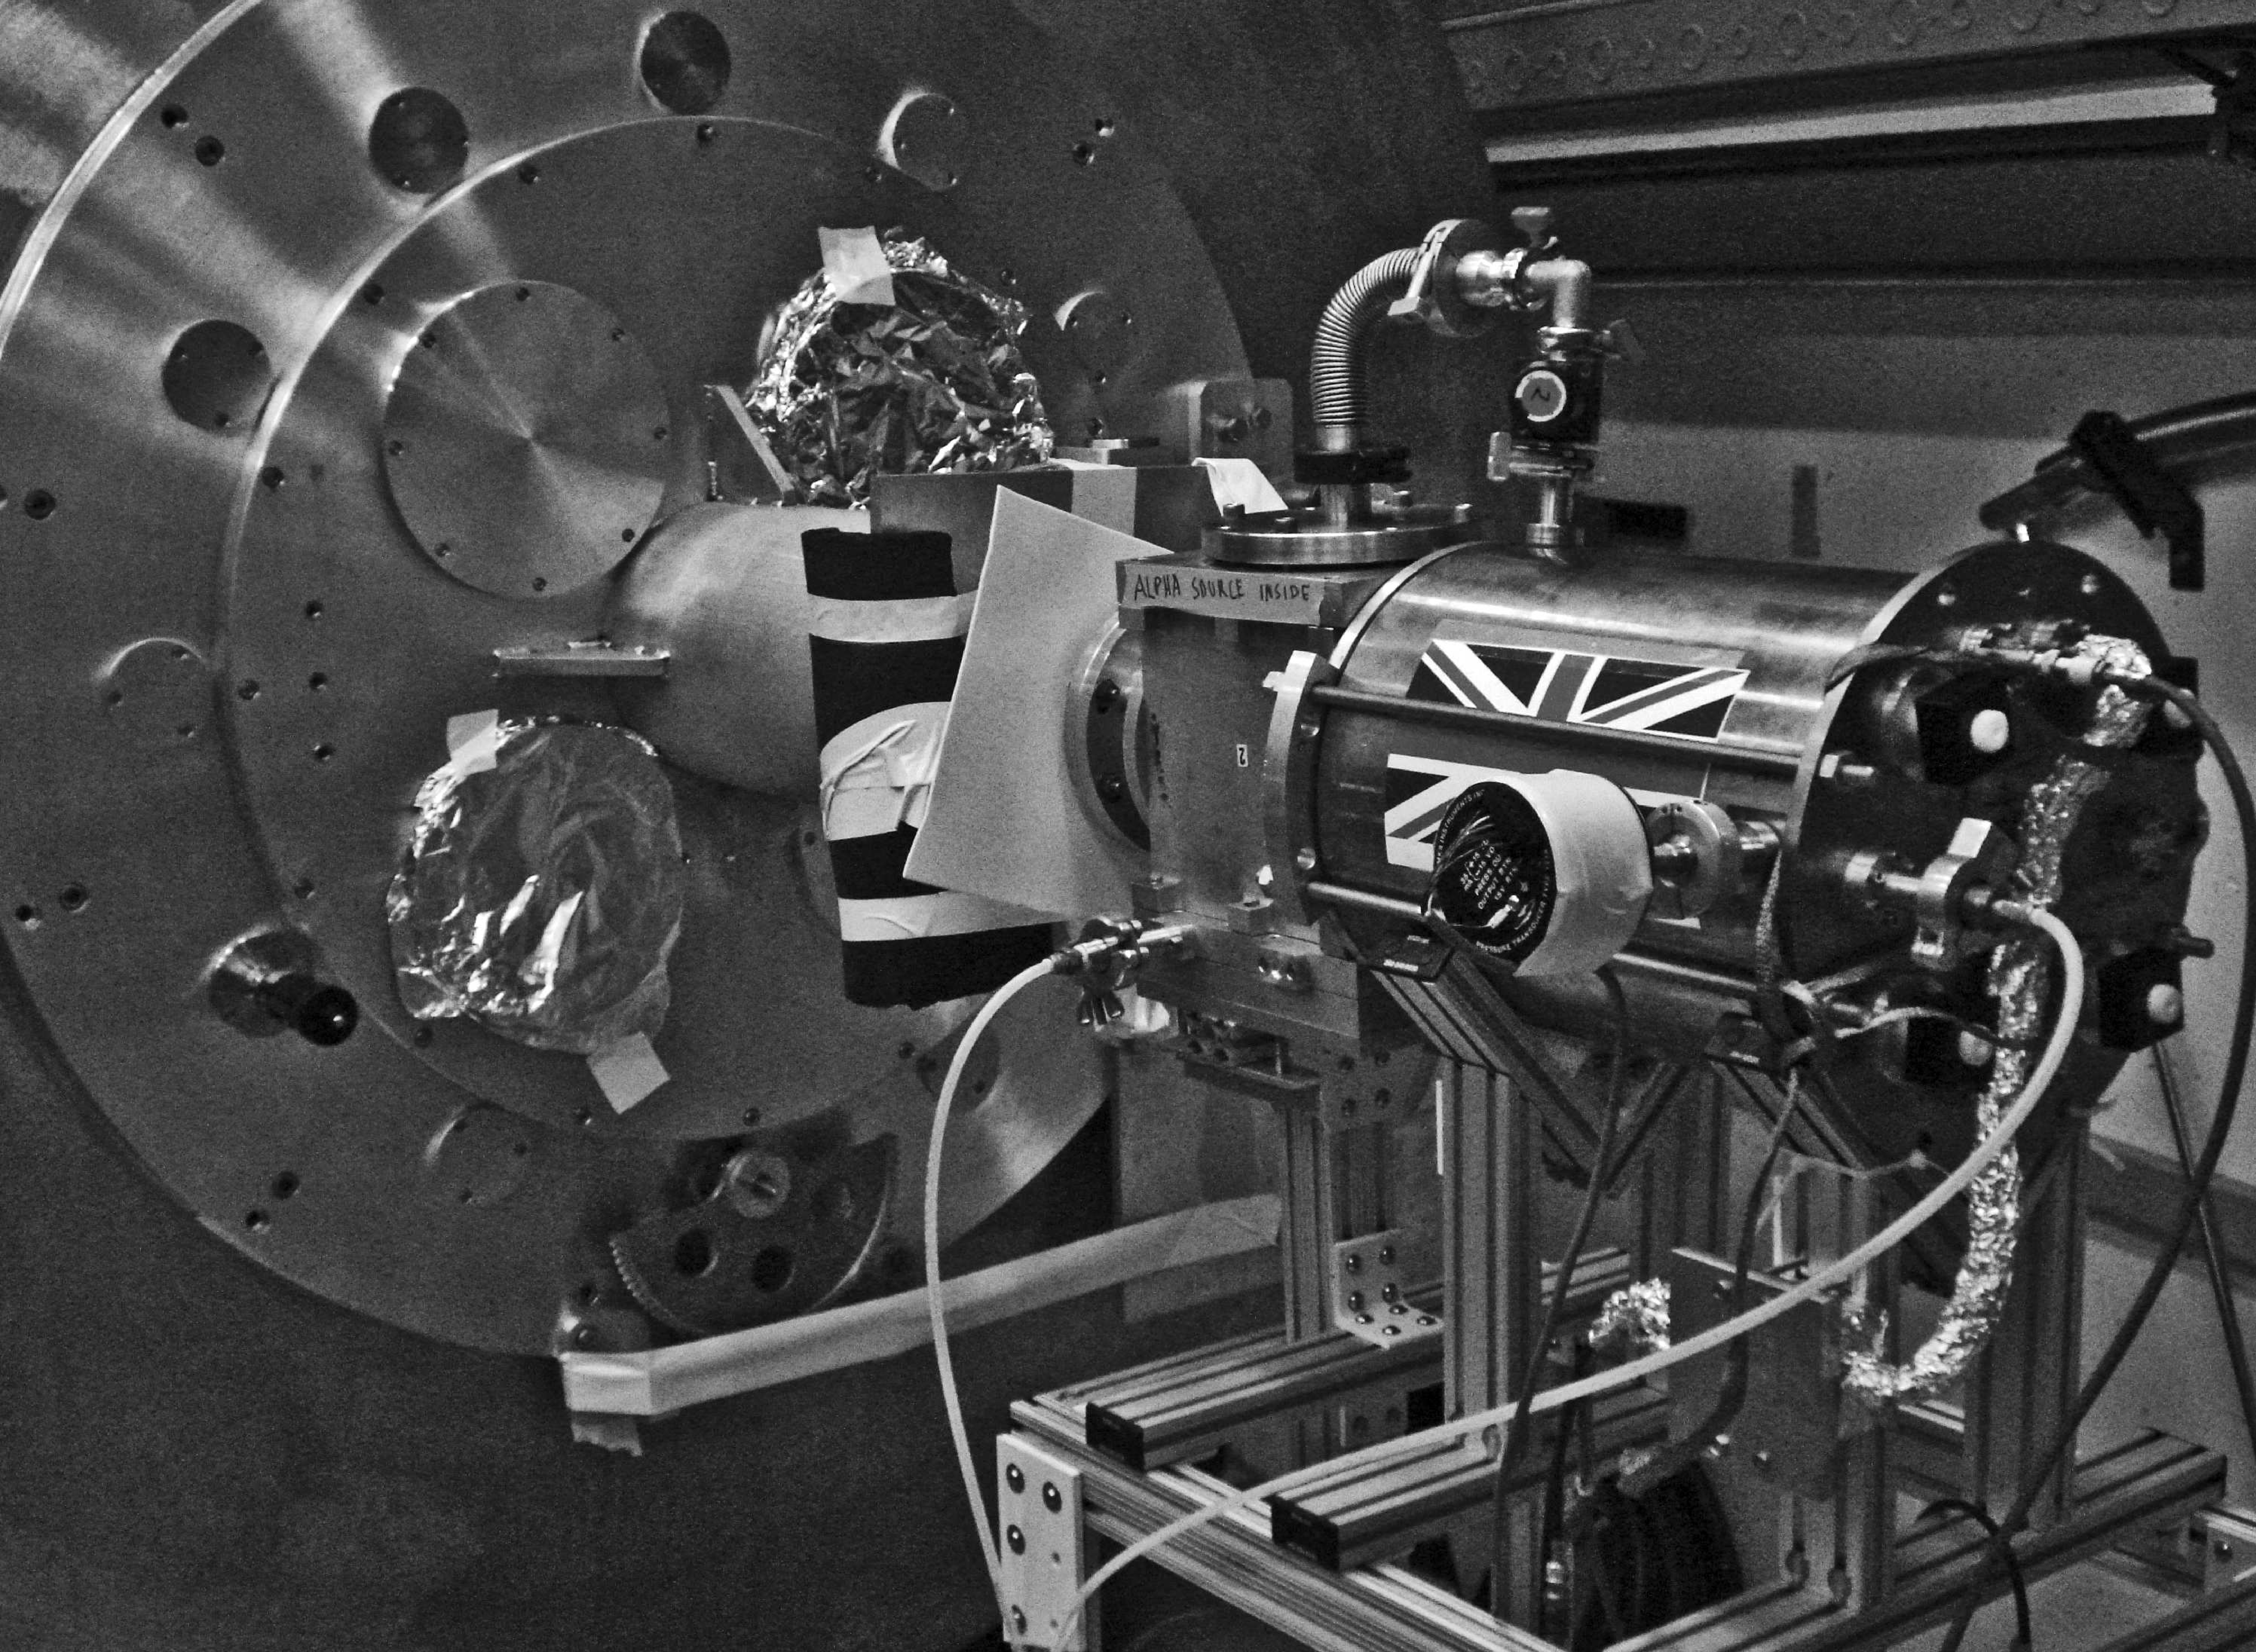
\includegraphics[width=0.45\textwidth,height=0.3\textheight,keepaspectratio]{DSC01964}
\caption[Gas-filled recoil detectors for HELIOS]{Gas-filled recoil detectors for HELIOS.  (Left) Schematic drawing of the redesigned downstream HELIOS door including the Bragg curve detector (exterior) and a PPAC detector (interior).  Drawing by A.\ Smith. (Right) Magnetic field testing of a Bragg curve detector during an energizing procedure of the HELIOS solenoid.}%In the photograph the Bragg curve detector is supported by a test stand.  In the design of the new rear door, the Bragg curve detector will be retrofitted to the door, occupying the volume currently currently occupied by the beam pipe flange.
\label{bragg}%
\end{figure}
%\subsection{PPAC}
%\section{Decay Detection}
%\subsection{}
%e$^+$e$^-$ pair detection Inelastic proton scattering from $^{12}$C to study the branching ratio of the 5\,MeV 0$^+$\ ``Hoyle State'' \ldots a continuation of an earlier measurement \cite{Tur_2006,Tur_2008,Goodman_2009}.
%\subsection{}
%possible future plans for $\gamma$-ray detection
%\enlargethispage{8pt}%required to maintain page numbering with \linenumbers